\documentclass[10pt,pdf,hyperref={unicode}]{beamer}

% \documentclass[aspectratio=43]{beamer}
% \documentclass[aspectratio=1610]{beamer}
% \documentclass[aspectratio=169]{beamer}

\usepackage{lmodern}

% подключаем кириллицу 
\usepackage[T2A]{fontenc}
\usepackage[utf8]{inputenc}

\usepackage[utf8]{inputenc}
\usepackage[russian]{babel}
\usepackage{cmap}

\setbeamertemplate{caption}[numbered]

\usepackage{graphicx}
\graphicspath{{pictures/}}
\DeclareGraphicsExtensions{.pdf,.png,.jpg}


% отключить клавиши навигации
\setbeamertemplate{navigation symbols}{}

% тема оформления
\usetheme{boxes}

% цветовая схема
\usecolortheme{seahorse}

\title{Кто лучше <<Westeros Inc>> или <<Harpy \& Co>>?}   
\subtitle{Анализ качества стали}
\author{
Мареев Глеб, Меледин Станислав, Сударева Лера, Шуган Алёна} 
\date{20 апреля 2018 года} 
% \logo{\includegraphics[height=5mm]{images/logo.png}\vspace{-7pt}}



\begin{document}

% титульный слайд
\begin{frame}
\titlepage
\end{frame} 

\begin{frame}
\frametitle{Метод} 
\framesubtitle{}
Для составления рекомендаций: какого поставщика стали выбрать, необходимо найти сильные стороны каждого поставщика. 

Сделаем это посчитав различные статистики и построив их графики для каждой компании.

После этого поймем: какого поставщика в каком случае нужно выбирать.
\end{frame}


\begin{frame}
\frametitle{Сильные стороны <<Westeros Inc>>} 
\framesubtitle{}

\begin{minipage}{0.4\textwidth}
 	\begin{figure}[L]
		\center{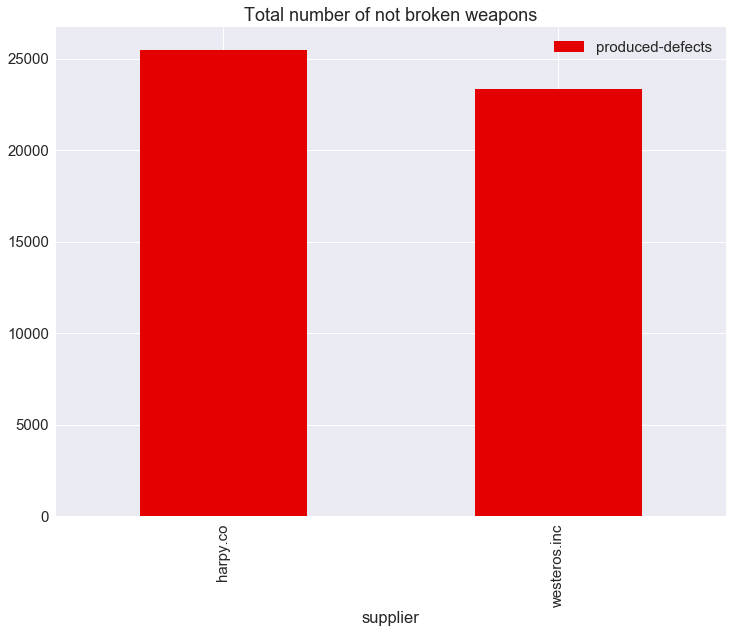
\includegraphics[width=180px]{12.png}}
		\caption{Общее число несломанных мечей}	
	\end{figure}
\end{minipage}
\hfill
\begin{minipage}{0.4\textwidth}
	По объему несломанных мечей, изготовленных из стали, лидирует компания <<Westeros Inc>>.
\end{minipage}
\end{frame}

\begin{frame}
\frametitle{Сильные стороны <<Westeros Inc>>} 
\framesubtitle{}

\begin{minipage}{0.4\textwidth}
 	\begin{figure}[L]
		\center{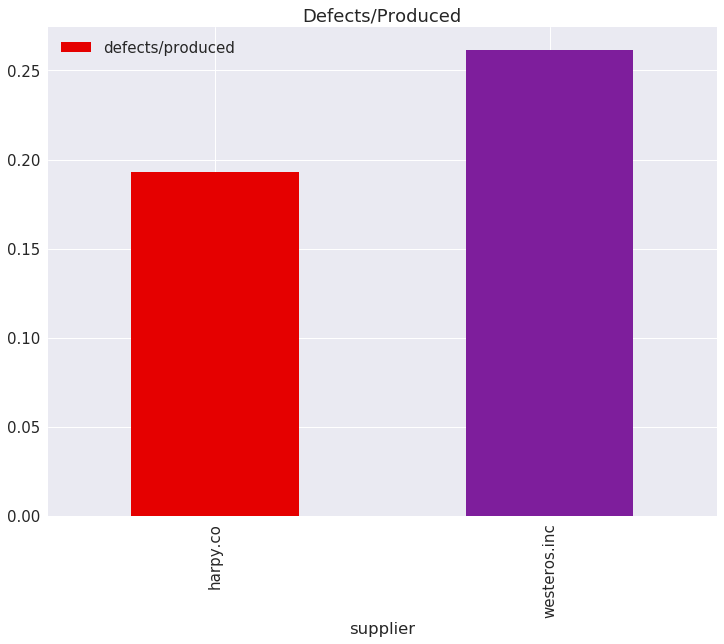
\includegraphics[width=180px]{2.png}}
		\caption{Отношения числа сломанных мечей к произведенным}		
	\end{figure}
\end{minipage}
\hfill
\begin{minipage}{0.4\textwidth}
	У компании <<Westeros Inc>> меньший процент отношения $\frac{\text{Кол-во сломанных мечей}}{\text{Кол-во произведенных мечей}}$.
\end{minipage}
\end{frame}

\begin{frame}
\frametitle{Сильные стороны <<Westeros Inc>>} 
\framesubtitle{}

\begin{minipage}{0.4\textwidth}
 	\begin{figure}[L]
		\center{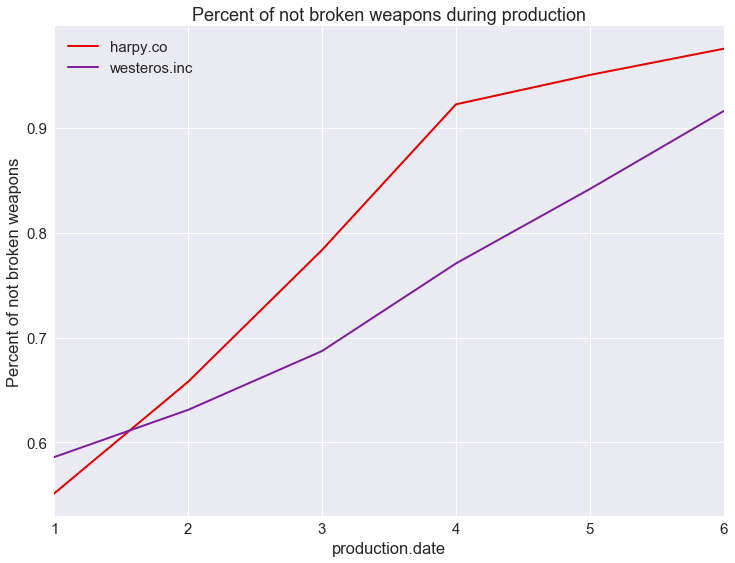
\includegraphics[width=180px]{11.png}}
		\caption{Общее число несломанных мечей с течением времени}		
	\end{figure}
\end{minipage}
\hfill
\begin{minipage}{0.4\textwidth}
	Из стали компании <<Westeros Inc>> мечи производят быстрее.
\end{minipage}
\end{frame}

\begin{frame}
\frametitle{Сильные стороны <<Harpy \& Co>>} 
\begin{minipage}{0.4\textwidth}
 	\begin{figure}[L]
		\center{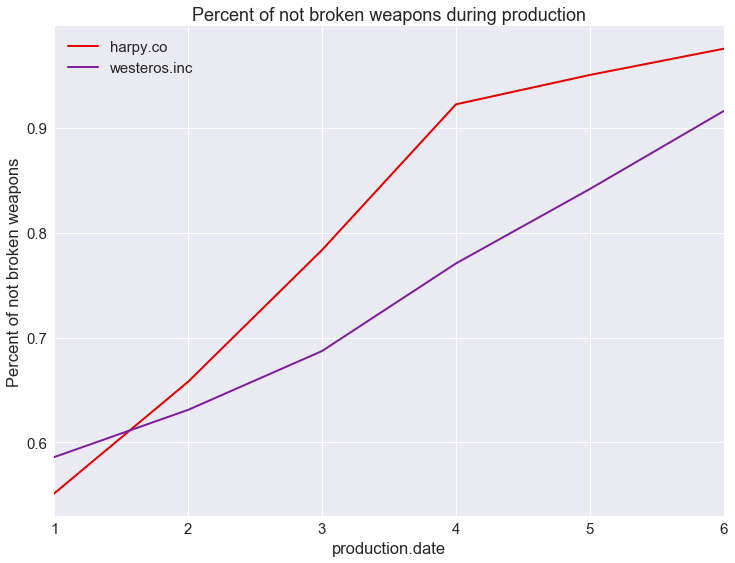
\includegraphics[width=180px]{11.png}}
		\caption{Общее число несломанных мечей с течением времени}
	\end{figure}
\end{minipage}
\hfill
\begin{minipage}{0.4\textwidth}
	Стабильность роста количества несломанных мечей из стали <<Harpy \& Co>>.
\end{minipage}
\end{frame}

\begin{frame}
\frametitle{Сильные стороны <<Harpy \& Co>>} 
\begin{minipage}{0.4\textwidth}
 	\begin{figure}[L]
		\center{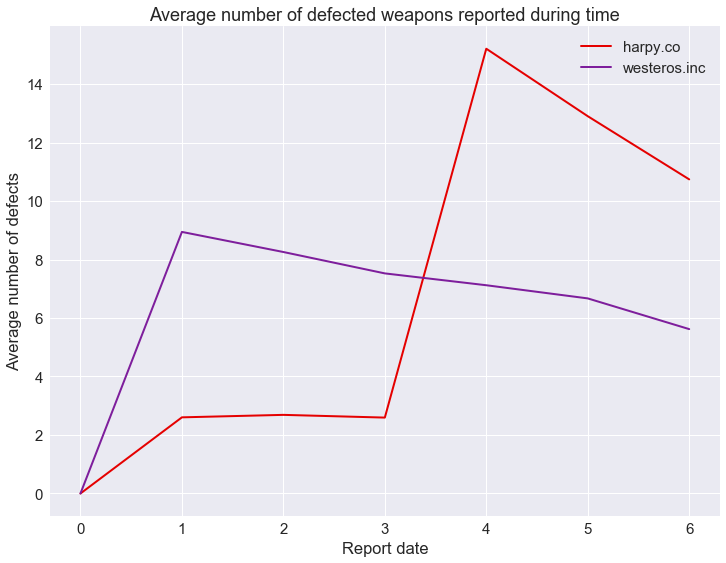
\includegraphics[width=180px]{3.png}}
		\caption{Среднее число сломанных мечей с течением времени}
	\end{figure}
\end{minipage}
\hfill
\begin{minipage}{0.4\textwidth}
	Уменьшение числа сломанных мечей, произведенных из стали  <<Harpy \& Co>>, с течением времени.
\end{minipage}
\end{frame}

\begin{frame}
\frametitle{Выводы} 

В итоге пришли к следующим выводам:
\begin{itemize}
\item Если нужно срочно увеличить количество вооружения, то необходимо выбрать компанию <<Westeros Inc>>, но за скорость придется платить: с течением времени число сломанных мечей увеличится.
\item Если есть время для подготовки, то лучше выбрать компанию <<Harpy \& Co>>, так как их продукция более качественная, а дефекты выявляются на ранних этапах.
\end{itemize}
\end{frame}

\end{document}